%\TODO{Observed fit results: support note 9.7 p. 138}

After running the full analysis chain, the event yields in the signal region, low-$m_{jj}$ control region, and $WZ$ control region as well as associated nuisance parameters representing the uncertainties are passed to the maximum likelihood fit.
From this fit, the normalization factor for the $WZ$ control region $\mu_{WZ}$ and the signal strength parameter in the signal region $\mu_{\textrm{obs}}$ are determined, and the predicted yields in each input bin have been shifted according to the process detailed in Section~\ref{ssww13tev:xsec_fit_method}.

The $WZ$ normalization factor is measured to be:
\begin{equation}
  \mu_{WZ} = 0.88^{+0.07}_{-0.07}(\textrm{stat})~^{+0.31}_{-0.21}(\textrm{theory})~^{+0.22}_{-0.11}(\textrm{sys})
  \label{eq:ssww13tev_signal_strength_wz}
\end{equation}
and is constrained primarily by the number of data events in the $WZ$ control region.
The observed signal strength of \ssww EWK production, defined in Equation~\ref{eq:ssww13tev_xsec_mu}, is extracted from the fit and measured with respect to the prediction of the \sherpav{2.2.2} MC generator:
\begin{equation}
  \mu_{\textrm{obs}} = 1.45^{+0.25}_{-0.24}(\textrm{stat})~^{+0.06}_{-0.08}(\textrm{theory})~^{+0.27}_{-0.22}(\textrm{sys}) % paper has no theory uncert for some reason
  \label{eq:ssww13tev_signal_strength_sr}
\end{equation}
This corresponds to a rejection of the background-only hypothesis with a significance of $6.9\sigma$.

The observed number of data events are compared to the predicted signal and background yields in the signal region in Table~\ref{tab:ssww13tev_yields_prefit} before applying the fit and in Table~\ref{tab:ssww13tev_yields_postfit} after the fit.
122 candidate events are observed compared to a prediction of 60 signal and 69 background events.

The $m_{jj}$ distributions for data and prediction are shown in Figure~\ref{fig:ssww13tev_results_mjj_sr_postfit} after the fit, and the fitted event yields in the low-$m_{jj}$ and $WZ$ control regions are shown in Figure~\ref{fig:ssww13tev_results_cr_postfit}.
Additional distributions can be found in Appendix~\ref{app:ssww13tev_additional_material}.

\begin{table}[htbp]
  \resizebox{\linewidth}{!}{
  \begin{tabular}{l|l@{$\,\pm\,$}ll@{$\,\pm\,$}ll@{$\,\pm\,$}ll@{$\,\pm\,$}ll@{$\,\pm\,$}ll@{$\,\pm\,$}l|l@{$\,\pm\,$}l}
    & \multicolumn{2}{c}{$\eep$}& \multicolumn{2}{c}{$\eem$}& \multicolumn{2}{c}{$\mep$}& \multicolumn{2}{c}{$\mem$}& \multicolumn{2}{c}{$\mmp$}& \multicolumn{2}{c|}{$\mmm$}& \multicolumn{2}{c}{combined}\\
\hline\hline
$WZ$                    & 1.9 & 0.6 & 1.3 & 0.4 & 14 & 4 & 8.9 & 2.6 & 5.5 & 1.6 & 3.6 & 1.1 & 35 & 10 \\ % before scaling (calculated by hand)
Non-prompt            & 4.1& 2.3   & 2.3& 1.7   & 9& 5   & 6& 4   & 0.57& 0.15   & 0.67& 0.25   & 23& 10 \\
$e/\gamma$ conversions         & 1.74& 0.29   & 1.8& 0.4   & 6.1& 1.6   & 3.7& 0.8   & \multicolumn{2}{c}{---}   & \multicolumn{2}{c|}{---}   & 13.4& 2.5 \\
Other prompt          & 0.17& 0.05   & 0.14& 0.04   & 0.90& 0.19   & 0.60& 0.14   & 0.36& 0.10   & 0.19& 0.05   & 2.4& 0.5 \\
\ssww QCD              & 0.38& 0.13   & 0.16& 0.05   & 3.0& 1.0   & 1.2& 0.4   & 1.8& 0.6   & 0.76& 0.25   & 7.3& 2.5 \\
\hline
Expected background   & 8.2 & 2.4 & 5.7 & 1.8 & 33 & 7 & 21 & 5 & 8.2 & 1.8 & 5.3 & 1.2 & 81 & 14  \\
\hline
\ssww EWK & 3.8 & 0.6 & 1.49 & 0.22 & 16.5 & 2.5 & 6.5 & 1.0 & 9.1 & 1.4 & 3.5 & 0.5 & 41 & 6 \\
\hline
Data& \multicolumn{2}{c}{10}& \multicolumn{2}{c}{4}& \multicolumn{2}{c}{44}& \multicolumn{2}{c}{28}& \multicolumn{2}{c}{25}& \multicolumn{2}{c|}{11}& \multicolumn{2}{c}{122}\\
\hline
\end{tabular}
  }
  \caption{Table of the data and prediction event yields in the signal region before the fit.  Numbers are shown for the six lepton flavor and charge channels and for all channels combined.  Here the $WZ$ background yields are normalized to the data in the $WZ$ control region.  The background estimations from the fake-factor are included in the ``Non-prompt'' category, and backgrounds from  $V\gamma$ production and electron charge misidentification are combined in the ``$e/\gamma$ conversions'' category. Finally, $ZZ$, $VVV$, and $t\bar{t}V$ backgrounds are combined in the ``Other prompt'' category.}
  \label{tab:ssww13tev_yields_prefit}
\end{table}

\begin{table}[htbp]
  \resizebox{\linewidth}{!}{
    \begin{tabular}{l|l@{$\,\pm\,$}ll@{$\,\pm\,$}ll@{$\,\pm\,$}ll@{$\,\pm\,$}ll@{$\,\pm\,$}ll@{$\,\pm\,$}l|l@{$\,\pm\,$}l}
    & \multicolumn{2}{c}{$\eep$}& \multicolumn{2}{c}{$\eem$}& \multicolumn{2}{c}{$\mep$}& \multicolumn{2}{c}{$\mem$}& \multicolumn{2}{c}{$\mmp$}& \multicolumn{2}{c|}{$\mmm$}& \multicolumn{2}{c}{combined}\\
    \hline\hline
    $WZ$                    & 1.49& 0.30   & 1.10& 0.26   & 11.7& 1.7   & 8.0& 1.3   & 5.0& 0.6   & 3.5& 0.6   & 31& 4 \\
    Non-prompt            & 2.2& 1.3   & 1.2& 0.7   & 5.7& 2.8   & 4.5& 1.8   & 0.57& 0.06   & 0.65& 0.14   & 15& 6 \\
    $e/\gamma$ conversions           & 1.6& 0.4   & 1.6& 0.5   & 6.3& 1.6   & 4.3& 1.1   & \multicolumn{2}{c}{---} & \multicolumn{2}{c|}{---}   & 13.8& 2.9 \\
    Other prompt          & 0.16& 0.04   & 0.14& 0.04   & 0.90& 0.19   & 0.63& 0.13   & 0.39& 0.09   & 0.22& 0.05   & 2.4& 0.5 \\
    \ssww QCD              & 0.35& 0.13   & 0.15& 0.05   & 2.9& 1.0   & 1.2& 0.4   & 1.8& 0.6   & 0.76& 0.25   & 7.2& 2.4 \\
    \hline
    Expected background   & 5.8& 1.5   & 4.1& 1.1   & 27& 4   & 18.7& 2.6   & 7.7& 0.8   & 5.1& 0.6   & 69& 7 \\
    \hline
    \ssww EWK            & 5.6& 1.0   & 2.2& 0.4   & 24& 5   & 9.4& 1.8   & 13.5& 2.5   & 5.2& 1.0   & 60& 11 \\
    \hline
    Data& \multicolumn{2}{c}{10}& \multicolumn{2}{c}{4}& \multicolumn{2}{c}{44}& \multicolumn{2}{c}{28}& \multicolumn{2}{c}{25}& \multicolumn{2}{c|}{11}& \multicolumn{2}{c}{122}\\
    \hline
    \end{tabular}
  }
  \caption{Table of the data and prediction event yields in the signal region after the fit.  Numbers are shown for the six lepton flavor and charge channels and for all channels combined.  The background estimations from the fake-factor are included in the ``Non-prompt'' category, and backgrounds from  $V\gamma$ production and electron charge misidentification are combined in the ``$e/\gamma$ conversions'' category.  Finally, $ZZ$, $VVV$, and $t\bar{t}V$ backgrounds are combined in the ``Other prompt'' category.}
  \label{tab:ssww13tev_yields_postfit}
\end{table}

\begin{figure}[htbp]
  \centering
  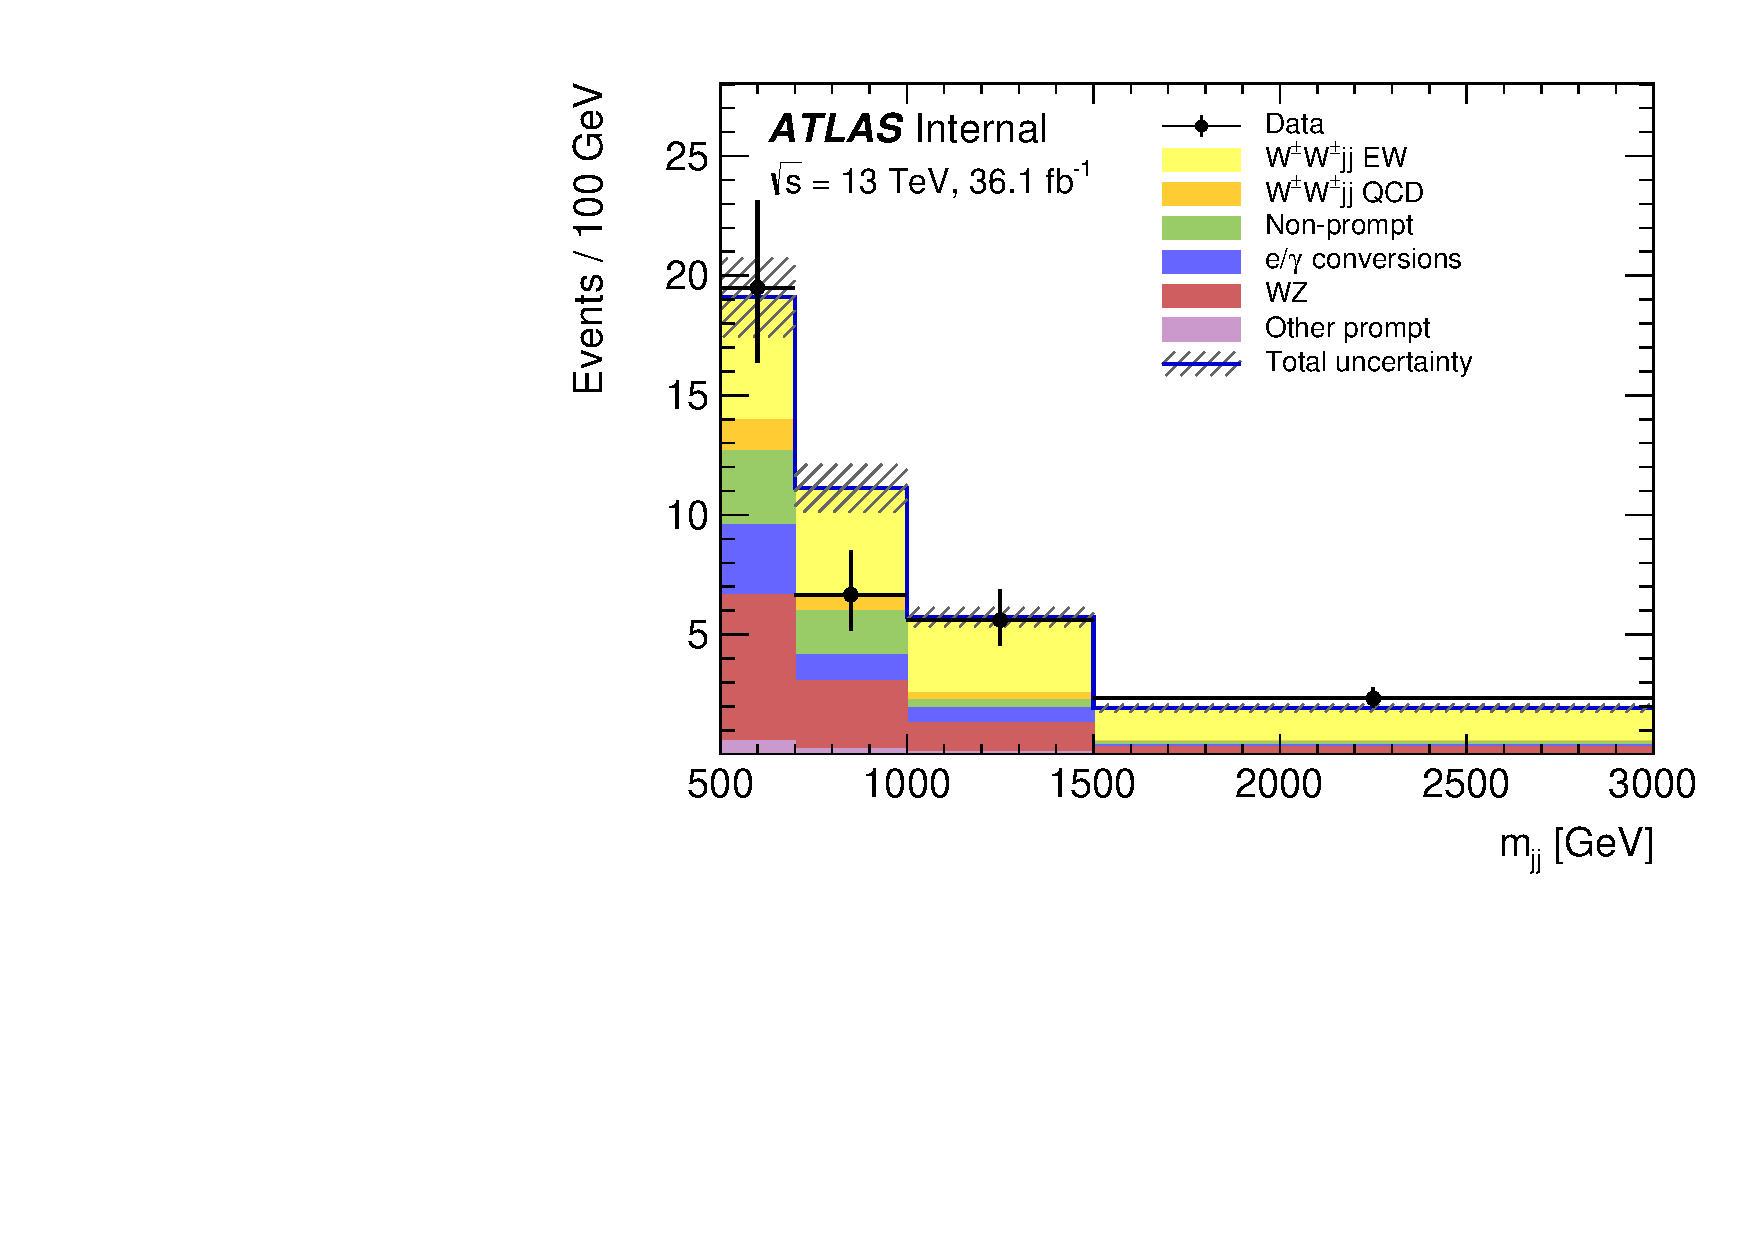
\includegraphics[width=.6\textwidth]{figs/ssww_13tev/results/mjj_postfit_all}
  \caption{The dijet invariant mass $m_{jj}$ distributions for data and predicted signal and background in the signal region after the fit.  The shaded band represents the statistical and systematic uncertainties added in quadrature.  Note that the bins have been scaled such that they represent the number of events per $100\gev$ in $m_{jj}$.  The background estimations from the fake-factor are included in the ``Non-prompt'' category, and backgrounds from  $V\gamma$ production and electron charge misidentification are combined in the ``$e/\gamma$ conversions'' category.  Finally, $ZZ$, $VVV$, and $t\bar{t}V$ backgrounds are combined in the ``Other prompt'' category.}
  \label{fig:ssww13tev_results_mjj_sr_postfit}
\end{figure}

\begin{figure}[htbp]
  \centering
  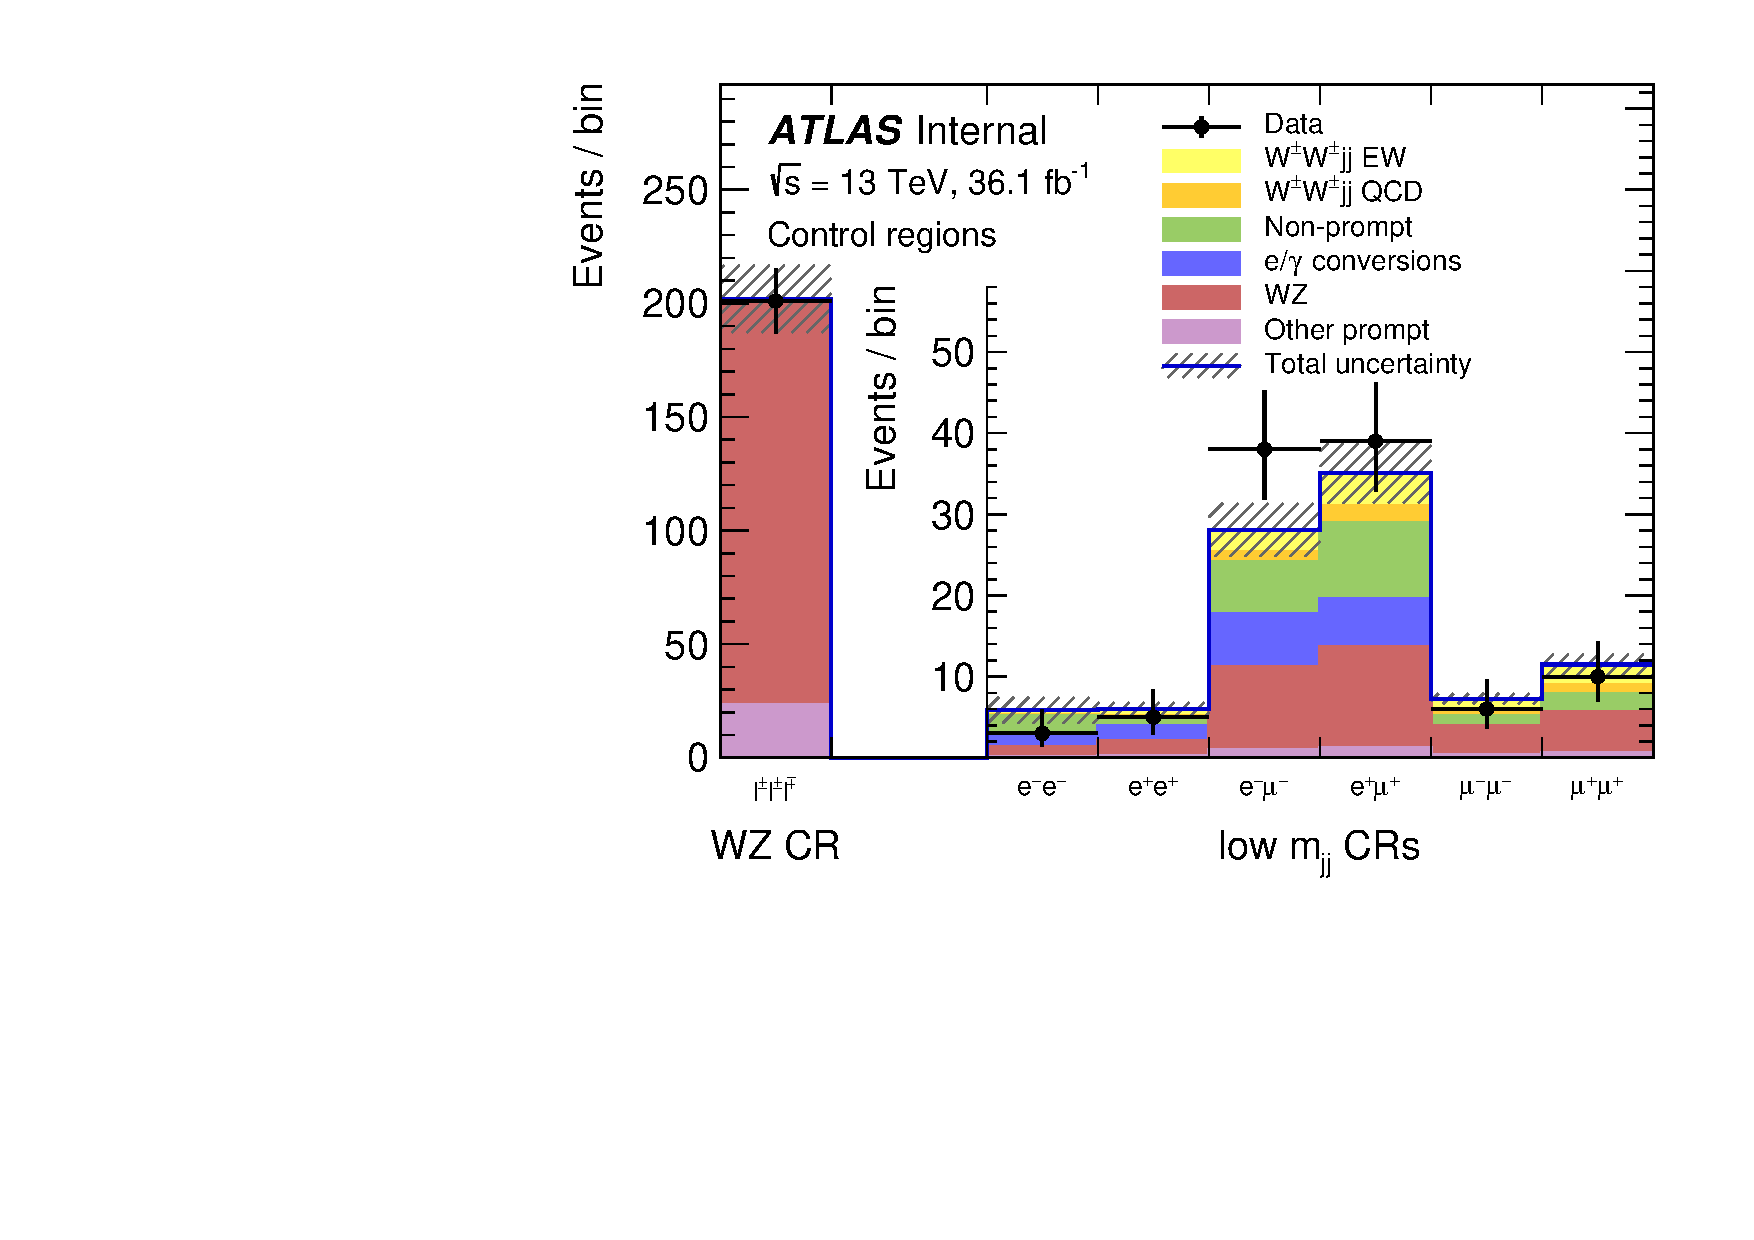
\includegraphics[width=.6\textwidth]{figs/ssww_13tev/results/plotCR}
  \caption{The event yields for data and predicted signal and background in the $WZ$ and low-$m_{jj}$ control regions after the fit.  The shaded band represents the statistical and systematic uncertainties added in quadrature.  The background estimations from the fake-factor are included in the ``Non-prompt'' category, and backgrounds from  $V\gamma$ production and electron charge misidentification are combined in the ``$e/\gamma$ conversions'' category.  Finally, $ZZ$, $VVV$, and $t\bar{t}V$ backgrounds are combined in the ``Other prompt'' category.}
  \label{fig:ssww13tev_results_cr_postfit}
\end{figure}

The last ingredient necessary to measure the \ssww EWK cross section is the theory predicted cross section in the fiducial region defined in Table~\ref{tab:ssww13tev_fiducial_vol}.
\sherpav{2.2.2} is used for the calculation, and the cross section in the total generator phase space is $40.81\pm 0.05~\textrm{fb}$, and the fiducial cross section is $2.01\pm 0.02~\textrm{fb}$.
This corresponds to an acceptance factor of $\mathcal{A} = 0.0493\pm 0.0002$.
Uncertainties on the simulation are estimated using variations of the scale, parton shower, and PDF set.
The final prediction used in the cross section measurement including uncertainties from Section~\ref{ssww13tev:theory_uncert} is:
\begin{equation}
  \sigma_{\tt{SHERPA}}^{\textrm{fid}} = 2.01 \pm 0.02(\textrm{stat})~^{+0.29}_{-0.23} (\textrm{scale})~^{+0.16}_{-0.02}(\textrm{parton shower})~^{+0.05}_{-0.03} (\textrm{PDF})~\textrm{fb}
  \label{eq:ssww13tev_fiducial_xsec_theory}
\end{equation}

Combining this \tt{SHERPA} prediction with the measured signal strength $\mu_{\textrm{obs}}$ from Equation~\ref{eq:ssww13tev_signal_strength_sr}, the measured fiducial cross section $\sigma_{\textrm{meas}}^{\textrm{fid}}$ can be calculated using Equation~\ref{eq:ssww13tev_xsec_fid_meas_mu}:
\begin{equation}
  \sigma_{\textrm{meas}}^{\textrm{fid}} = 2.91^{+0.51}_{-0.47}(\textrm{stat})~^{+0.12}_{-0.16}(\textrm{theory})~^{+0.24}_{-0.23}(\textrm{sys})~^{+0.08}_{-0.06}(\textrm{luminosity})~\textrm{fb}
  \label{eq:ssww13tev_fiducial_xsec}
\end{equation}
A plot comparing the measured fiducial cross section to two theoretical calculations is shown in Figure~\ref{fig:ssww13tev_results_xsec}.
The measured value is compared to the \sherpav{2.2.2} prediction used to calculate $\mu_{\textrm{obs}}$ as well as to \powhegbox{2}.
As mentioned in Section~\ref{ssww13tev:mc}, this \tt{POWHEG} sample does not include the resonant triboson diagrams and is only used here for a visual comparison.

\begin{figure}[htbp]
  \centering
  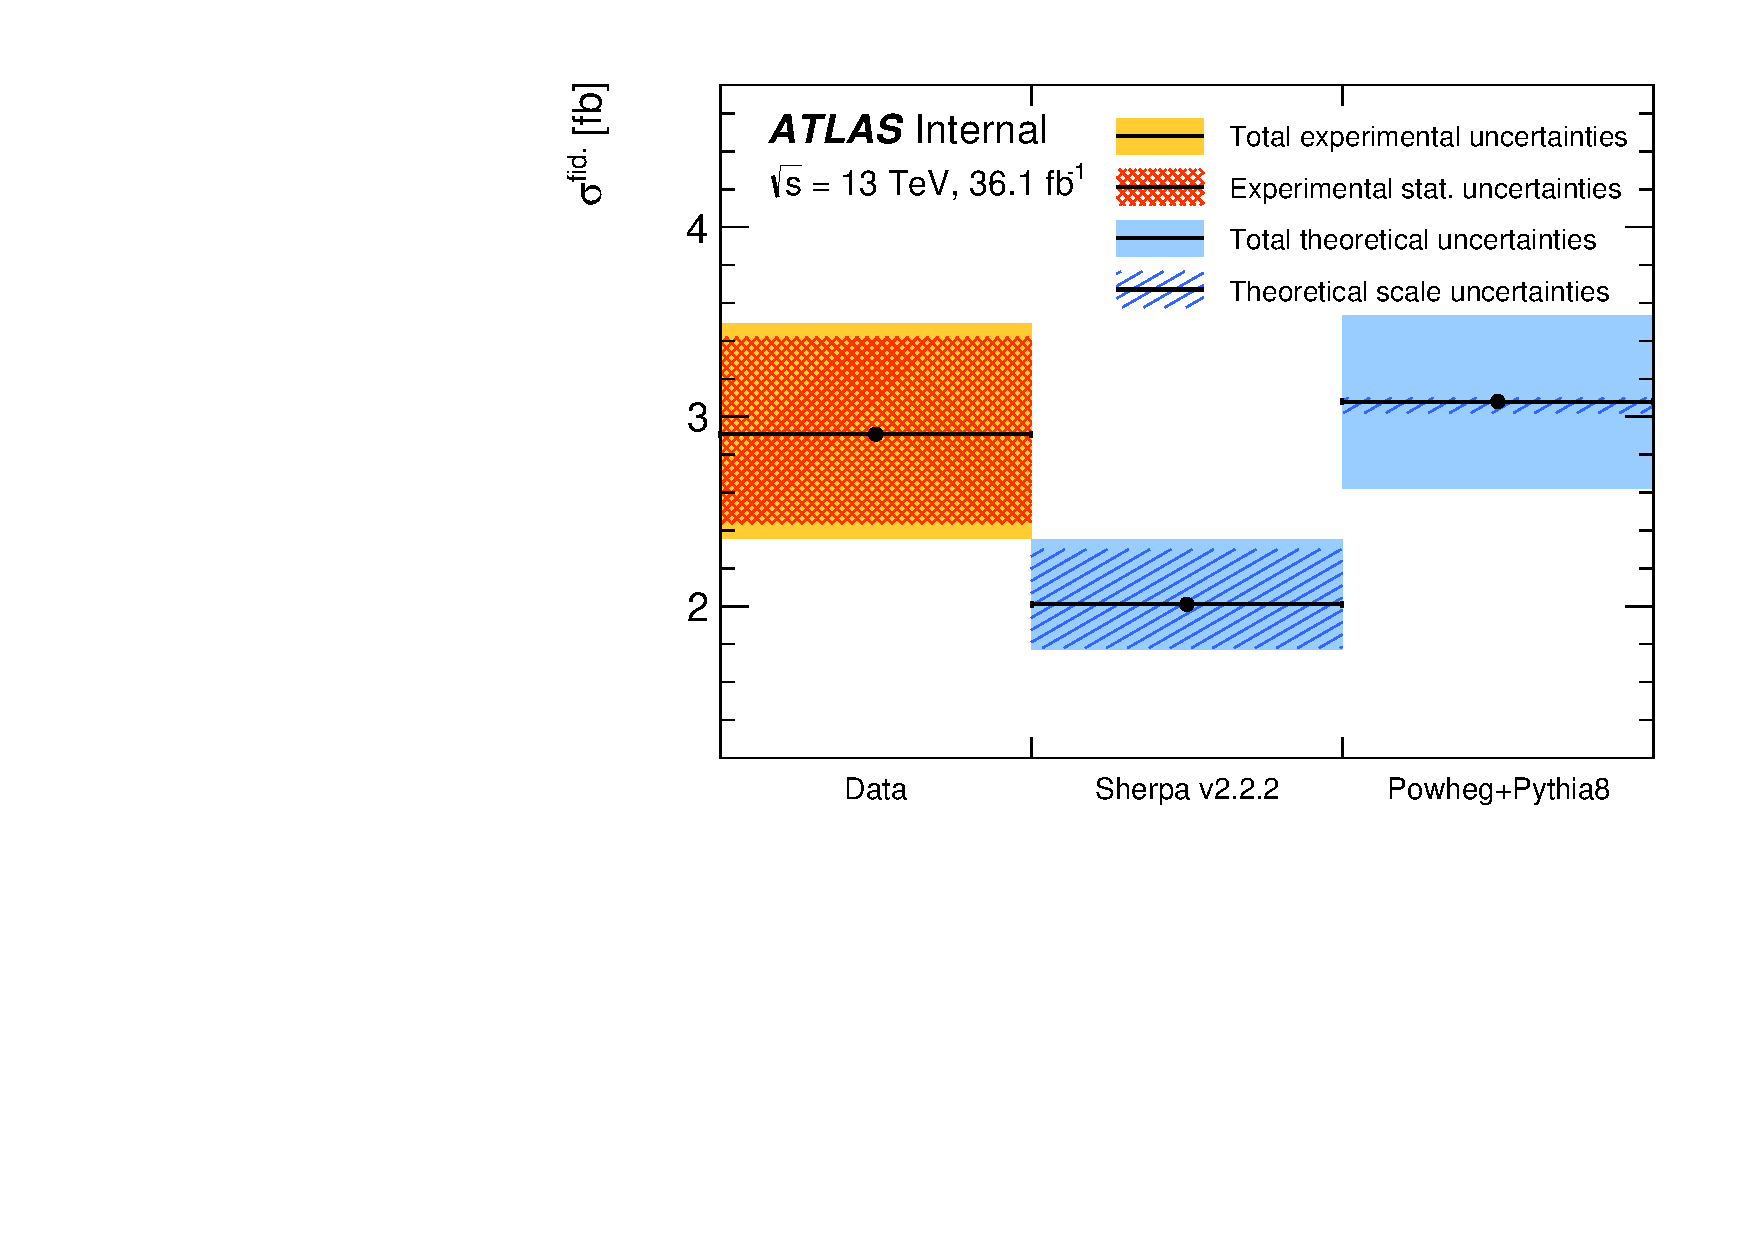
\includegraphics[width=.6\textwidth]{figs/ssww_13tev/results/NP_post_fit__xsec_ExpObs}
  \caption{Comparison of the measured \ssww EWK fiducial cross section with theoretical calculations from \sherpav{2.2.2} and \powhegbox{2}.  The light orange band represents the total experimental uncertainty on the measured value, and the dark orange hashed band is the statistical uncertainty.  For the simulations, the light blue band represents the total theoretical uncertainty, and the dark blue hashed band are the scale uncertainties.  The theory predictions do not include the interference between the EWK and QCD production.}
  \label{fig:ssww13tev_results_xsec}
\end{figure}
